\newcommand{\pa}{CH$_3$CNH$^+$ }
\newcommand{\pan}{CH$_3$CNH$^+$}

\section*{Abstract}
The gas phase vibrational spectrum of \pa is recorded using a messenger infrared predissociation (IRPD) action spectroscopic method. Vibrational bands were recorded in the $300-1700$~\wnn and $2000-3300$~\wnn regions making use of the widely tunable free electron laser for infrared experiments, FELIX, coupled to a cryogenic ion trap instrument. Band assignments were aided by high-level quantum-chemical calculations, which showed excellent agreement with the experimental data. Effects of the neon atom used as messenger in the IRPD method are investigated in detail. The data presented here will support astronomical searches for the \pa ion in space, and provides a basis for high-resolution ro-vibrational and pure rotational studies in vibrationally excited states.
\clearpage

\section{Introduction}

Methyl cyanide (CH$_3$CN, also known as acetonitrile) was among the first polyatomic molecules detected during radio-astronomical observations of the interstellar medium (ISM) \cite{SJP1971}. It has since been detected in a variety of galactic sources, covering most evolutionary stages from dense cold cores \cite{GMO2016,VLW2019}, via low- and high-mass star-forming regions \cite{AGM2018,FOG2015} and protoplanetary disks \cite{OGF2015} to photodissociation regions \cite{GPG2014} and circumstellar envelopes \cite{ACQ2015}. CH$_3$CN has also been detected in the atmosphere of Saturn's moon Titan \cite{MHB2002,Thelen2019AbundanceObservations,IST2020}.

As methyl cyanide has a proton affinity of $788(8)$~kJ/mol \cite{KFM1986}, much larger than that of H$_2$, its protonated version (\pan) might form effectively via exothermic proton transfer from H$_3^+$ to CH$_3$CN in the interstellar medium \cite{ILB1981}. Another effective formation pathway of protonated methyl cyanide is via radiative association of CH$_3^+$ and HCN. The latter pathway, followed by dissociative recombination, was suggested to be the major gas-phase route for the interstellar synthesis of methyl cyanide (and its isocyanide isomer) \cite{HM1979,DMH1985, VKH2008}. Despite its dominant role in the formation of the ubiquituous methyl cyanide molecule, previous searches for \pa in the interstellar medium were unsuccessful \cite{TAF1990}. Protonated methyl cyanide, as well as other protonated nitriles, have, however, been detected in Titan's upper atmosphere by the Ion Neutral Mass Spectrometer (INMS) on board the Cassini spacecraft \cite{VYA2006}. It is dominantly formed by protonation of CH$_3$CN via reactions with the highly abundant ions HCNH$^+$ and C$_2$H$_5^+$, whose deprotonated variants have a lower proton affinity than methyl cyanide \cite{VYM2007}.

The pure rotational spectrum of protonated methyl cyanide has been studied extensively in the microwave \cite{GAM2000} and submillimeter-wave region \cite{AHH2006}.
Several infrared studies on \pa exist, including matrix-isolation FT-IR \cite{Frankowski2005} of its CH and NH stretching bands, infrared-predissociation (IRPD) action spectroscopy of its complex with H$_2$ in the H$_2$ and NH stretching region \cite{DRO1999}, and high-resolution gas-phase absorption spectroscopy on the $\nu_1$ NH stretching fundamental band of the bare ion \cite{Amano1988, Amano1992}. All these studies focus on the stretching bands located at wavelengths below 3.4~$\mu$m, or at wavenumbers above 2900~\wn, respectively, and to date no spectroscopic data on its low-lying vibrational modes existed.

In this study we recorded the vibrational spectrum of gas-phase \pa over a broad frequency range  ($300-1700$ and $2000-3300$~\wn) covering all fundamental modes except the previously studied NH stretching band. Experiments were performed using Ne-tagging infrared-predissociation spectroscopy in a cryogenic ion trap coupled to the powerful and widely tunable FELIX (Free Electron Lasers for Infrared eXperiments, \cite{oepts_free-electron-laser_1995}) free-electron IR lasers. These data can serve as reference data for future laboratory infrared studies at high spectral resolution as well as astronomical searches for this important ion in space, e.g., with the upcoming James Webb Space Telescope (JWST). 


\section{Methods}

\subsection{Experimental details}

\begin{figure}
	\centering
		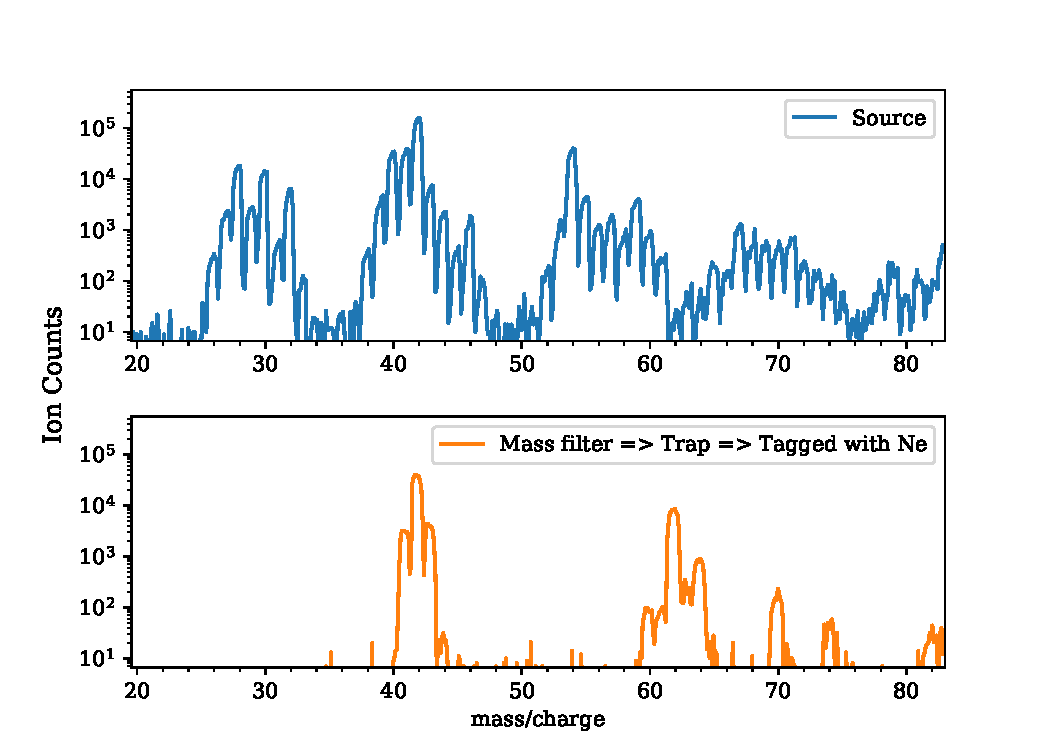
\includegraphics[scale=.6]{chapters/CH3CNH+/figures/masspec_log.pdf}
	\caption{Upper panel: Mass spectra of ions produced from electron impact ionization ($\sim$30eV) in a storage ion source. See text for discussion of the main peaks Lower panel: { Mass filtered \pa (m/z = 42, $<10$~\% contribution at m/z = 41 and 43) together with tagged \pan -Ne (m/z = 62, also \pan -$^{22}$Ne at  m/z = 64) species produced in the cryogenic ion trap. Additional weaker contributions at m/z = 60, 70, and 74 stem from tagging with residual H$_2$O, N$_2$, and O$_2$, respectively.}  }
	\label{FIG:CH3CNH+:masspec}
\end{figure}

The vibrational spectrum of \pa was recorded using the FELion cryogenic 22-pole ion trap instrument.  A detailed account of the FELion instrument is provided in Section \ref{sec:felion} and the infrared-predissociation (IRPD) of in-situ rare gas tagged cold molecular ions in Section \ref{subsec:action:methods:vibrational:IRPD}. Here we only give a brief account of details specific to the \pa ion.

Protonated methyl cyanide (m/z = 42) was produced by electron impact ionization (EI, electron energy 30~eV) from neutral methyl cyanide (Sigma Aldrich, $>99.9$\%) in a Gerlich-type storage ion source (SIS) \cite{Gerlich1992}, where primary ions produced by EI are accumulated for the duration of an experimental cycle (of the order of seconds). { The precursor gas was admitted either pure or diluted with He at a ratio of 1:3 to the ion source chamber at a pressure of $\sim 10^{-5}$~mbar. Self-protonation of the primarily formed methyl cyanide radical cations with neutral methyl cyanide \cite{TFI2010}, led to effective production of \pa (see Figure \ref{FIG:CH3CNH+:masspec}). Additional prominent mass-peaks in the mass-spectrum are due to the radical methyl cyanide cation (m/z = 41) and the hydrogen loss fragment CH$_2$CN$^+$ with m/z = 40. Interestingly, we observe the appearance of a mass-peak at m/z = 54, which is likely caused by a reaction of CH$_2$CN$^+$ with neutral methyl cyanide in the storage source \cite{ATF2012}. Fragment ions, including their protonated  forms are apparent in the range m/z = $26 - 32$, contamination from water and air leads to additional contributions at m/z = 18 (not shown), 28, and 32.} 

For spectroscopic IRPD experiments a few 10~ms long pulse of ions is extracted from the source and filtered for the mass of interest, m/z = 42 in the case of \pa by a quadrupole mass filter before entering the 22-pole ion trap which is held at a fixed temperature in the range 6.1-7~K for experiments using Ne as tagging gas. Around 10-20~ms before the ions enter the trap, an intense 80-150~ms long Ne:He pulse (1:3 mixing ratio and number density of $\sim 10^{15}$~cm$^{-3}$) is admitted to the trap, leading to efficient collisional cooling of the ions to the ambient temperature. Under these conditions, { around 20~\% of the \pa ions form weakly bound complexes with Ne, see Figure \ref{FIG:CH3CNH+:masspec}.} The ions are stored for several seconds in the ion trap and are exposed to several laser pulses before extraction. An IR-PD spectrum is recorded by mass-selecting and counting the \pan-Ne complex ions while tuning the laser frequency $\nu$. A relative depletion $D=1-\frac{N_{ON}(\nu)}{N_{OFF}}$ in the number of complex ions $N_{ON}(\nu)$ from the baseline value $N_{OFF}$ is observed upon resonant vibrational excitation. To account for varying laser pulse energy $P$, pulse number $n$, and for saturation effects, the signal is normalized prior to averaging using $I=\frac{- ln(N_{ON}(\nu)/N_{OFF})}{n\cdot P/(h\nu)}$, giving the intensity $I$ in units of relative cross-section per photon. 
After normalizing each measurement in this way, the final spectrum is then obtained by averaging using statistical binning with a typical bin size of 2.5~\wn. Line parameters such as band positions, intensities, and line widths (fwhm) are then obtained by fitting a multi-component Gaussian function to the experimental data, also providing statistical errors of the line parameters.


The vibrational IRPD spectra were recorded using the IR radiation of FEL-2 of the FELIX Laboratory in the frequency region 300-1700 \wn, and in the range 2000-3300 \wnn employing the $3^{rd}$ harmonic mode of the FEL. The laser was operated at 10~Hz with macro pulse energies in the interaction region between 1.5-60~mJ, and for each datapoint $n=$3-66 pulses were admitted depending on the signal strength. The FEL was optimized for narrow bandwidth with a full width at half-maximum (fwhm) of $0.3-1$~\% of the center wavelength.\\

\subsection{Computational details} 

\begin{figure}
	\centering
		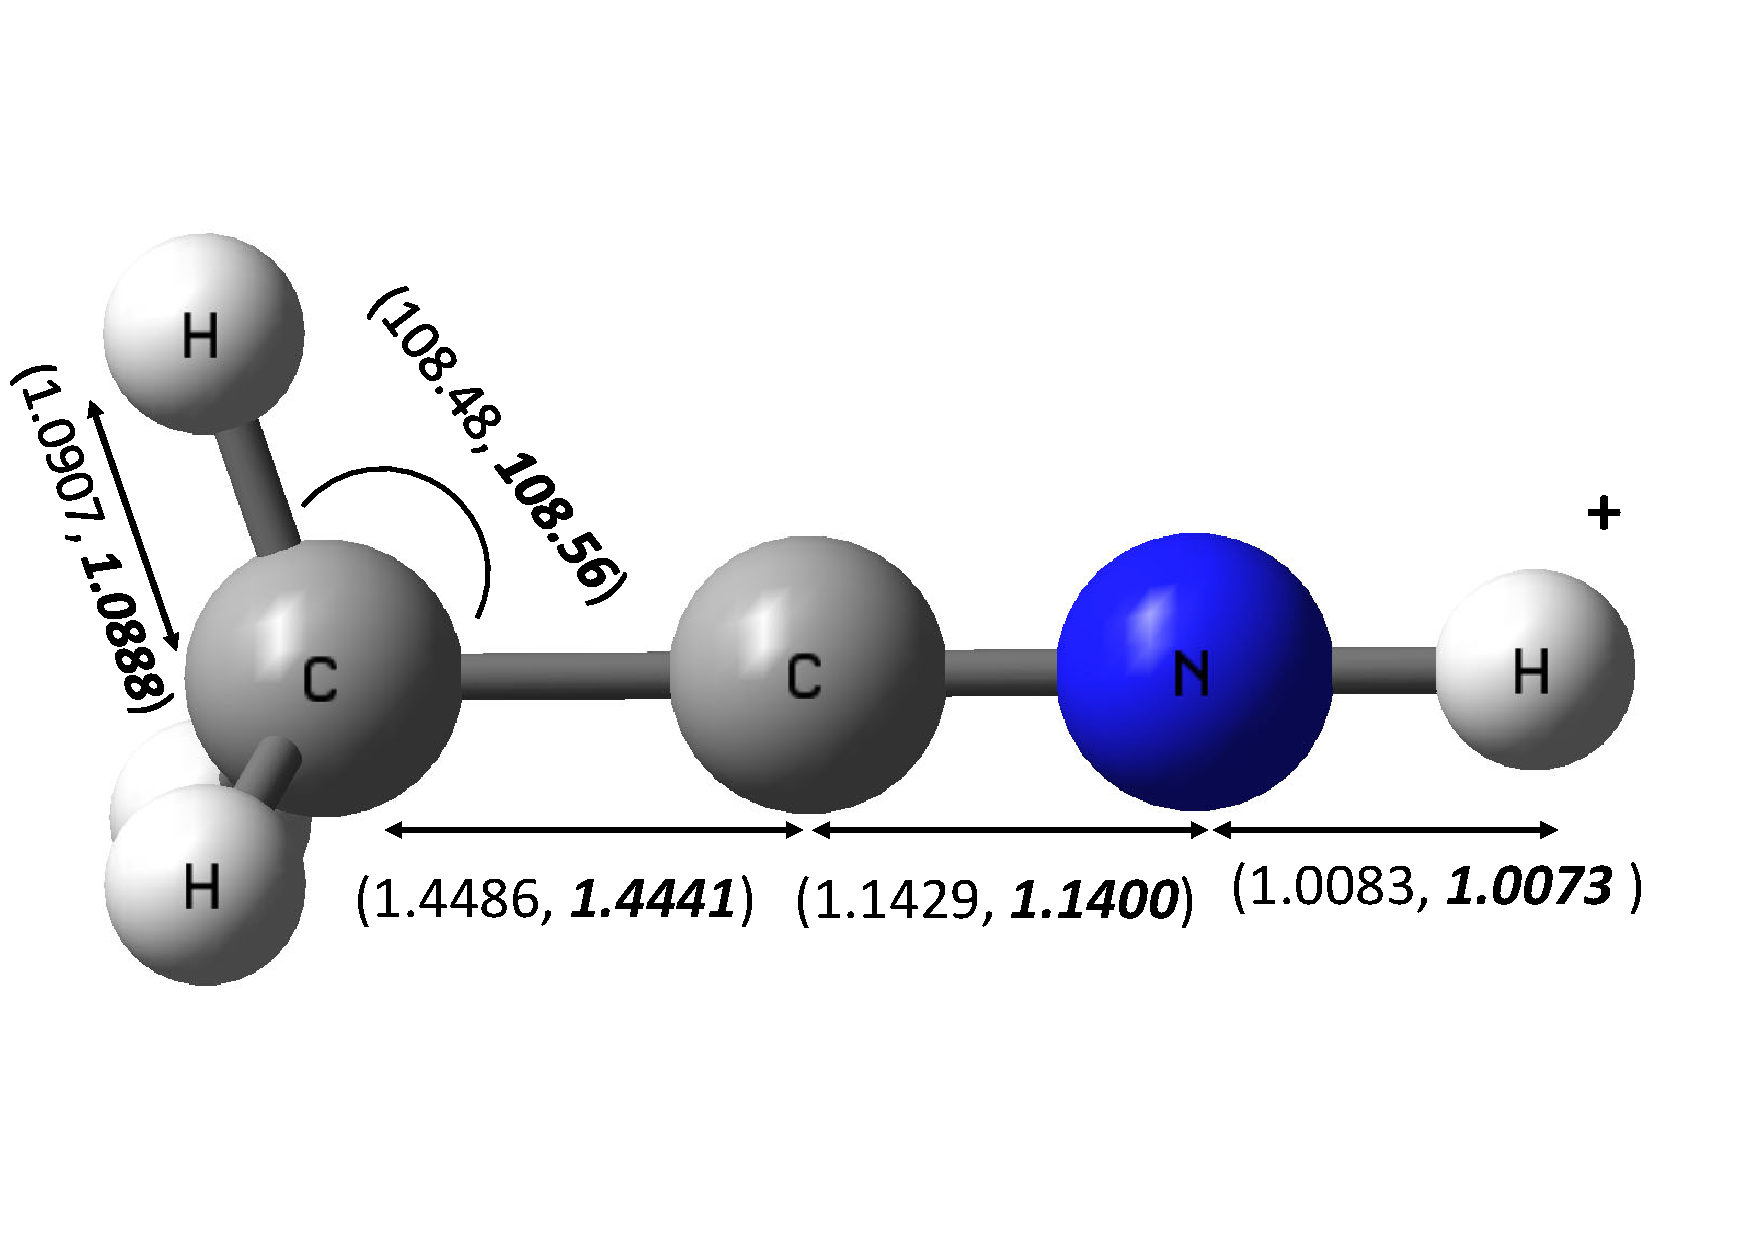
\includegraphics[scale=.3]{chapters/CH3CNH+/figures/molecule.pdf}
		\caption{Computed equilibrium geometry (C$_{3v}$ symmetry) for \pa based on (fc-CCSD(T)/ANO2, \textbf{\textit{ae-CCSD(T)/cc-pwCV5Z}}) level of theory. Bond lengths and angles are in $\mathring{A}$ and deg$^{\circ}$ respectively.}
	\label{FIG:molecule}
\end{figure}

The stability and relative energies of the [C$_2$H$_4$N]$^+$ isomeric family have been extensively studied previously at various levels of theory, showing N-protonated acetonitrile (\pa, $^1A_1$, C$_{3v}$ symmetry) to be the global minimum structure \cite{wuerthwein_1984, Cerqueira2020}.
In the present study we have investigated \pa at the coupled-cluster singles and doubles (CCSD) level augmented by a perturbative treatment of triple excitations, CCSD(T)  \cite{raghavachari_chemphyslett_157_479_1989}, in combination with atomic natural orbital (ANO0, ANO1, and ANO2) basis sets from Alml\"of and Taylor \cite{almlof_JCP_86_4070_1987} as well as the
correlation-consistent valence basis set cc-pVDZ \cite{dunning_gaussian_1989}
in the frozen core (fc) approximation. A best estimate equilibrium structure has been calculated using the cc-pwCV5Z basis set \cite{peterson_JCP_117_10548_2002} using all electrons in the correlation treatment.
Equilibrium geometries of \pa have been calculated using analytic gradient techniques  \cite{watts_chemphyslett_200_1-2_1_1992} and our results for the bare ion (Figure \ref{FIG:molecule}) match well with an earlier report by Botschwina \cite{Botschwina2000} who employed ab initio methods up to the CCSD(T)/cc-pCVQZ level. Harmonic frequencies were subsequently computed by numerical differentiation of
gradients \cite{lee_analytic_1991,watts_coupledcluster_1993}.
For anharmonic calculations, second-order vibrational perturbation theory (VPT2) \cite{mills_alphas} has been employed. All calculations have been carried out using the CFOUR program package  \cite{cfour_JCP_2020,harding_parallel_2008}. The CCSD(T) method in combination with ANO basis sets has been shown previously to provide vibrational wavenumbers of high quality  \cite{mccaslin_MolPhys_111_1492_2013,thorwirth_JMS_251_220_2008}, and we have recently applied it successfully for a vibrational study of [C$_3$H$_3]^+$ isomers and isotopologues \cite{Marimuthu2020LaboratorySpectroscopy}.

Additionally, we have performed potential energy scans to find the lowest energy structure of \pa complexed with Ne, as outlined in Section \ref{Neon influence}. These studies were conducted at the CCSD(T)/cc-pVDZ and CCSD(T)/ANO0 level of theory using the PSI4 program package \cite{PBL2017}. The potential energy surface as a function of H-Ne distance of the lowest energy conformer was then further investigated to account for Basis Set Superposition Errors \cite{liu_accurate_1973} using i) the counter-poise (CP) method introduced by Boys and Bernardi \cite{boys_calculation_1970}, i.e. by calculating CP-corrected CCSD(T) interaction energies at each geometry, and ii) higher-order symmetry-adapted perturbation theory, SAPT2+3/cc-pVDZ  \cite{jeziorski_perturbation_1994, hohenstein_density_2010}. In all PES calculations the geometry of the bare ion was kept fixed to its equilibrium structure calculated at the same level of theory. No zero-point vibrational energy (ZPE) corrections were applied to the derived binding energies.

\section{Results and discussions}
\subsection{Vibrational spectroscopy of \texorpdfstring{\pa}{CH3CNH+}}

\begin{figure}
	\centering
		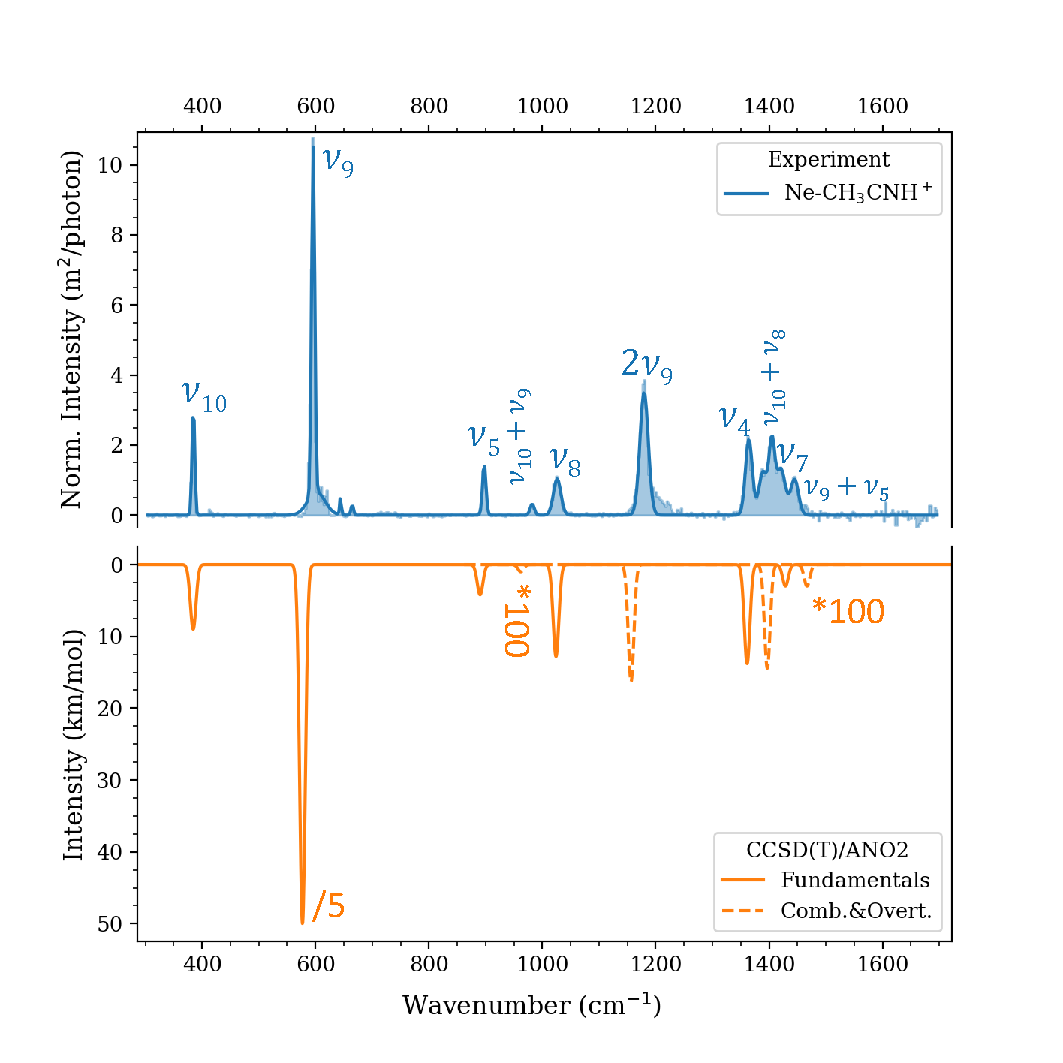
\includegraphics[scale=.7]{chapters/CH3CNH+/figures/felix_1_rev.pdf}
	\caption{The experimental and fitted FELIX IRPD spectrum of \pan-Ne (upper panel) compared to the computed anharmonic (VPT2) frequency values (lower panel) of \pa at the fc-CCSD(T)/ANO2 level of theory showing fundamental (orange, solid line), combination and overtone (orange, dashed line) bands. NOTE: /n and *n indicates that the computed intensities are divided or multiplied, respectively, by a  factor n for better visualisation }
	\label{FIG:felix_1}
	
\end{figure}

\begin{figure}
	\centering

		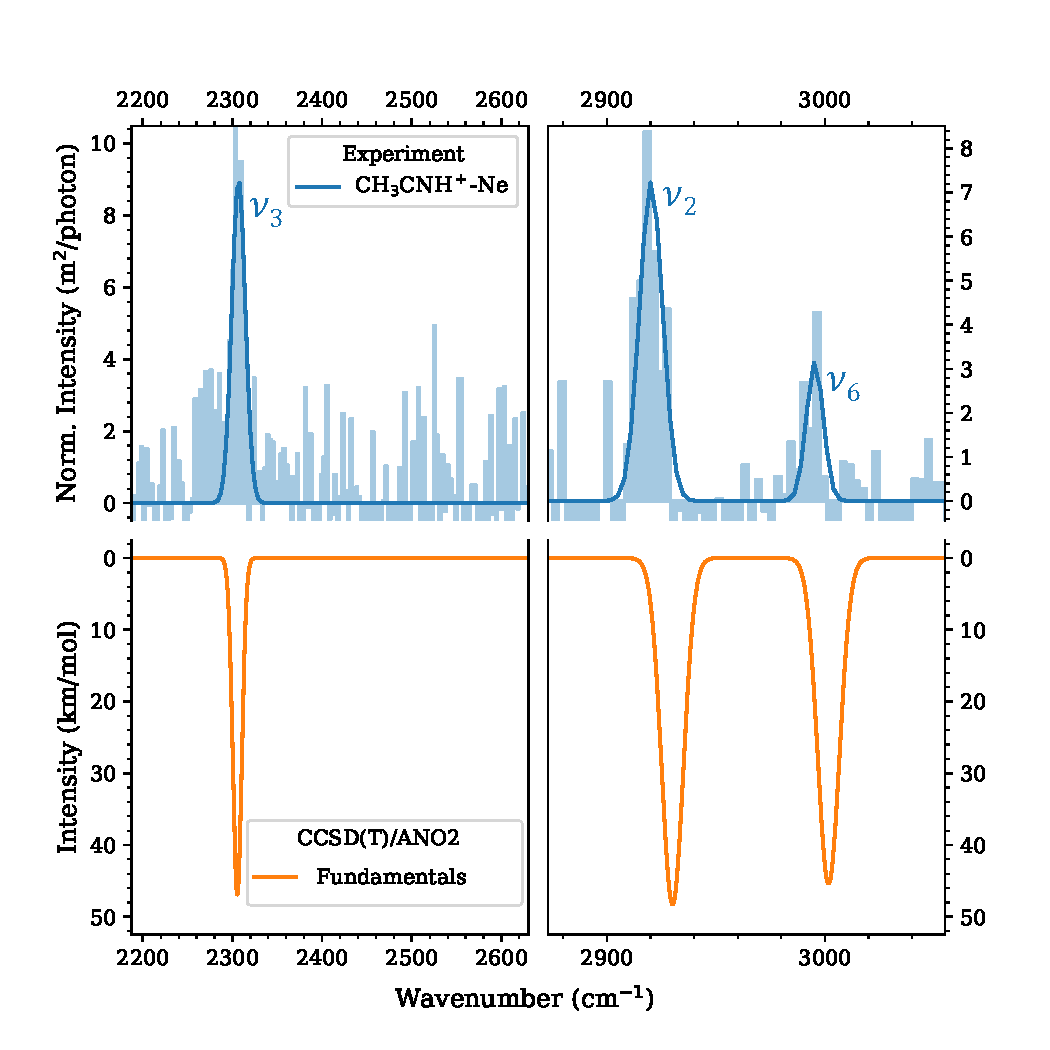
\includegraphics[scale=.7]{chapters/CH3CNH+/figures/felix_2_edited.pdf}
	\caption{The experimental and fitted FELIX IRPD spectrum of \pan-Ne (upper panel) but using FELIX in 3$^{rd}$ harmonic mode, compared to the computed anharmonic (VPT2) frequency values (lower panel) of \pa at the (fc)-CCSD(T)/ANO2 level of theory.}
	\label{FIG:felix_2}
	
\end{figure}

The measured IRPD spectra for [C$_2$H$_4$N]$^+$  with Ne as a tagging agent are displayed in Figures \ref{FIG:felix_1} and \ref{FIG:felix_2}, compared to the calculated spectrum of the energetically lowest lying isomer, \pan. Based on these results we can infer that only the most stable isomer \pa, i.e. N-protonated methyl cyanide, is produced via self-protonation in our storage ion-source. By exposing the complexes to $>100$ FEL shots on resonance with the strong band at 898~\wnn we could verify that $>95$\% of the complexes dissociate, i.e. that only one isomeric variant absorbing at this specific frequency is present in the ion trap. The \pa structure with C$_{3v}$ symmetry has 10 IR active fundamental modes of E and A$_1$ symmetry. As can be clearly seen in Figure \ref{FIG:felix_1} and \ref{FIG:felix_2}, we have covered and assigned all fundamental modes, except the high-lying NH-stretching mode that was out of the range of the FEL. Four remaining weak to moderately strong features could be assigned to combination and overtone modes predicted by the anharmonic force field calculations. The fitted band positions and assignments are summarized in Table \ref{tbl1:CH3CNH+}.
Several remaining, weak features, e.g., between $600-700$~\wnn are likely due to combination bands of the bare ions fundamental modes and those involving the weakly bound Ne atom. The observed transitions for \pan-Ne are in very good agreement with the computed values of the  bare ion \pa (see Table \ref{tbl1:CH3CNH+}). For most bands the deviation is less than 10~\wn, except for the CNH bending mode, and the overtone and combination modes, as will be discussed below. The influence of the neon-tag on the vibrational band positions is discussed in more detail in section \ref{Neon influence}.

The lowest energy CCN bending mode $\nu_{10}$ is clearly observed at 385~\wn\\ with excellent agreement to the anharmonic predicted value at 384~\wn. The most prominent feature, the $\nu_9$ CNH bending mode, is observed at 596~\wn, almost 20~\wnn blue-shifted from the predicted band position of the bare ion. This shift is likely caused by the attached neon atom, that binds to the proton involved in this bending mode (see section \ref{Neon influence}). The combination band of these two bending modes (CCN and CNH) was also observed at 982~\wnn as a weak feature. Also a very clear feature of the CNH first overtone appears at 1179~\wn. In general the computed values for the combination and overtone modes are $10-20$~\wnn shifted with respect to the experimentally observed bands. The CC stretching frequency $\nu_5$ is measured at 898~\wnn with a $\sim7$~\wnn blue-shift from the predicted value 890~\wn. The weak combination mode of the CC stretching with the CNH bending mode also appears with sizable intensity at 1445~\wn. We could also clearly observe the CH$_3$ vibrations, i.e. the $\nu_8$ wagging and $\nu_7$ scissoring, at 1026 and 1421~\wnn respectively (see vibrational displacement vectors given in the Supplementary Information Figure \ref{fig:CH3CNH+:fig2}). The former also forms a combination mode with the CCN bending at 1405~\wnn which matches well with the predicted value at 1397~\wnn (intensity over $14$~km/mol). The $\nu_4$ CH$_3$ umbrella like bending mode appears at 1364~\wnn very close to the predicted value at 1361~\wn. The $\nu_3$ CN stretching,  CH$_3$ $\nu_2$ symmetric and $\nu_6$ asymmetric stretching bands were measured with FELIX 3$^{rd}$ harmonic mode (see Figure \ref{FIG:felix_2}) resulting in lower resolution and signal-to-noise spectra, reflected in the larger experimental error of these lines. In addition, measurements of the two CH stretching bands suffered from calibration issues of the grating spectrometer used to determine the FEL frequency, reflected in their large systematic errors of 10~\wn.

\clearpage
\begin{landscape}
\begin{ThreePartTable}
    \begin{TableNotes}\footnotesize
        \item [a] \pa \& \pan-Ne (C$_{3v}$ symmetry isomer) harmonic frequencies were computed at the  CCSD(T)/ANO0 level of theory and their differences were added as Neon contribution to \pa frequencies computed at CCSD(T)/ANO2 (see section \ref{Neon influence}).\\
        \item [b] Frequencies (error in parentheses). nc indicates not covered.\\
        \item [c] Ne-matrix, Ref \cite{Frankowski2005}\\
        \item [d] Gas-phase, Ref \cite{Amano1992}\\
     \end{TableNotes}
    \begin{longtable}{*{16}{c}}

    \caption{Summary of IRPD experimental vibrational band position of \pan-Ne and comparison to computed values. Vibrational frequencies are in \wn [calc. intensities in km/mol]}\label{tbl1:CH3CNH+}\\

        \toprule
        \multicolumn{3}{c}{Vibrational symmetry and mode} & \multicolumn{2}{c}{CCSD(T)/ANO2} & Ne-IRPD\tnote{b} & prev. work   \\
            \multicolumn{3}{c}{(\pa, C$_{3v}$, $^1$A$_1$ ground state)} & (VPT2, anh.) & Ne corrected\tnote{a} &(this work) & \\\\
            \hline\\
            \multicolumn{3}{l}{Fundamental bands}&&\\\cline{1-3}\\
        
        \midrule
        \endfirsthead
        \\\\\hline \multicolumn{8}{c}{{\bfseries \tablename\ \thetable{} -- continued from previous page}} \\
        \toprule
        \multicolumn{3}{c}{Vibrational symmetry and mode} & \multicolumn{2}{c}{CCSD(T)/ANO2} & Ne-IRPD\tnote{b} & prev. work   \\
            \multicolumn{3}{c}{(\pa, C$_{3v}$, $^1$A$_1$ ground state)} & (VPT2, anh.) & Ne corrected\tnote{a} &(this work) & \\\\
            \hline\\
            \multicolumn{3}{l}{Fundamental bands}&&\\\cline{1-3}\\
    
        \toprule
        \endhead
    
        \midrule
        \insertTableNotes
        \\\\\hline \multicolumn{8}{c}{{\bfseries \tablename\ \thetable{} -- continued on next page}} \\ \hline
        \endfoot
        \bottomrule
        % \insertTableNotes
        \endlastfoot
            
            
            $\nu_{10}$ & E     & CCN bend            & 384  [4.5]    & 386  & 385  (1)  & \\
            $\nu_{9}$ & E      & CNH bend            & 577  [132.3]  & 595  & 596  (1)  & \\
            $\nu_5$ & A$_1$    & CC str.             & 890  [4.2]    & 891  & 898  (1)  & \\
            $\nu_8$ & E        & CH$_3$ wagging      & 1024 [6.4]    & 1025 & 1026 (1)  & \\
            $\nu_4$ & A$_1$    & CH$_3$ umbrella     & 1361 [13.8]   & 1362 & 1364 (1)  & \\
            $\nu_7$ & E        & CH$_3$ scissoring   & 1429 [1.5]    & 1429 & 1421 (1)  & \\
            $\nu_3$ & A$_1$    & CN str.             & 2305 [46.9]   & 2305 & 2307 (2)  & \\
            $\nu_2$ & A$_1$    & CH3 sym. str.       & 2930 [48.3]   & 2930 & 2924 (10) & \\
            $\nu_6$ & E        & CH3 asym. str.      & 3002 [22.7]   & 3002 & 2996 (10) & 2946.5 [53]\tnote{c} \\
            $\nu_1$ & A$_1$    & NH str.             & 3525 [654.7]  & 3516 & nc        & 3500.6 [677]\tnote{c}, 3527.29\tnote{d} \\
            \\
            \multicolumn{3}{l}{Overtones and Combination bands}&&\\\cline{1-3}\\\\
            $\nu_{10}+\nu_9$  & A$_1$& CCN bend + CNH bend     & 962 [0.01]  & & 982 (2) \\
            $2\nu_{9}$       & A$_1$& CNH bend (2)            & 1157 [16.3] & & 1179 (1)\\
            $\nu_{10}+\nu_8$  & A$_1$&  CCN bend + CH$_3$ wag  & 1397 [14.4] & & 1405 (1)\\
            $\nu_9+\nu_5$ & E & CC str. + CNH bend             & 1467 [0.03] & & 1445 (1)\\

    
    \end{longtable}
\end{ThreePartTable}
\end{landscape}
\clearpage
% \newgeometry{left=2cm}
% \begin{table}

%     \caption{Summary of IRPD experimental vibrational band position of \pan-Ne and comparison to computed values. Vibrational frequencies are in \wn [calc. intensities in km/mol]}\label{tbl1:CH3CNH+}
%         \centering
%         \small
%         \begin{tabular}{cccllrc}
    
%             \\\hline \hline\\
            
%             \multicolumn{3}{c}{Vibrational symmetry and mode} & \multicolumn{2}{c}{CCSD(T)/ANO2} & Ne-IRPD\textsuperscript{b} & prev. work   \\
%             \multicolumn{3}{c}{(\pa, C$_{3v}$, $^1$A$_1$ ground state)} & (VPT2, anh.) & Ne corrected$^a$ &(this work) & \\\\
%             \hline\\
%             \multicolumn{3}{l}{Fundamental bands}&&\\\cline{1-3}\\
            
%             $\nu_{10}$ & E     & CCN bend            & 384  [4.5]    & 386  & 385  (1)  & \\
%             $\nu_{9}$ & E      & CNH bend            & 577  [132.3]  & 595  & 596  (1)  & \\
%             $\nu_5$ & A$_1$    & CC str.             & 890  [4.2]    & 891  & 898  (1)  & \\
%             $\nu_8$ & E        & CH$_3$ wagging      & 1024 [6.4]    & 1025 & 1026 (1)  & \\
%             $\nu_4$ & A$_1$    & CH$_3$ umbrella     & 1361 [13.8]   & 1362 & 1364 (1)  & \\
%             $\nu_7$ & E        & CH$_3$ scissoring   & 1429 [1.5]    & 1429 & 1421 (1)  & \\
%             $\nu_3$ & A$_1$    & CN str.             & 2305 [46.9]   & 2305 & 2307 (2)  & \\
%             $\nu_2$ & A$_1$    & CH3 sym. str.       & 2930 [48.3]   & 2930 & 2924 (10) & \\
%             $\nu_6$ & E        & CH3 asym. str.      & 3002 [22.7]   & 3002 & 2996 (10) & 2946.5 [53]$^c$ \\
%             $\nu_1$ & A$_1$    & NH str.             & 3525 [654.7]  & 3516 & nc        & 3500.6 [677]$^c$, 3527.29$^d$ \\
%             \\
%             \multicolumn{3}{l}{Overtones and Combination bands}&&\\\cline{1-3}\\\\
%             $\nu_{10}+\nu_9$  & A$_1$& CCN bend + CNH bend     & 962 [0.01]  & & 982 (2) \\
%             $2\nu_{9}$       & A$_1$& CNH bend (2)            & 1157 [16.3] & & 1179 (1)\\
%             $\nu_{10}+\nu_8$  & A$_1$&  CCN bend + CH$_3$ wag  & 1397 [14.4] & & 1405 (1)\\
%             $\nu_9+\nu_5$ & E & CC str. + CNH bend             & 1467 [0.03] & & 1445 (1)\\
%             \\\hline\hline\\
%         \end{tabular}\\
    
%     $^a$ \pa \& \pan-Ne (C$_{3v}$ symmetry isomer) harmonic frequencies were computed at the  CCSD(T)/ANO0 level of theory and their differences were added as Neon contribution to \pa frequencies computed at CCSD(T)/ANO2 (see section \ref{Neon influence}).\\
%     $^b$ Frequencies (error in parentheses). nc indicates not covered.\\
%     $^c$ Ne-matrix, Ref \cite{Frankowski2005}\\
%     $^d$ Gas-phase, Ref \cite{Amano1992}\\
    
% \end{table}
% \restoregeometry
% \normalsize

\subsection{Prediction of rotational spectroscopic parameters}

The above discussion clearly shows that anharmonic calculations at the \\CCSD(T)/ANO2 level provide a reliable means to predict vibrational band positions for \pan. In addition, we present in Table \ref{tbl2} the calculated equilibrium and ground state rotational constants and compare the latter to experimentally derived values \cite{GAM2000,AHH2006} and a previous calculation using the aug-cc-pVQZ basis set \cite{Cerqueira2020}. 
From the relative deviations of the calculated spectroscopic constants to the experimental values, it is obvious that the fc-CCSD(T)/ANO2 calculation of $B_0$ (from the equilibrium rotational constant B$_e$ complemented by the zero point vibrational contribution $\Delta B_0$, see below) are slightly further off than the CCSD(T)/aug-cc-pVQZ values
reported earlier \cite{Cerqueira2020}, whereas centrifugal distortion constants show a similar accuracy. 
Best estimate ground state rotational constants have been calculated here using a hybrid approach with the equilibrium structure
calculated at the ae-CCSD(T)/cc-pwCV5Z and the zero-point vibrational corrections $\Delta B_{0}=\frac{1}{2}\sum{\alpha_i^B}$ (analogous for $A$) from rotation-vibration interaction constants $\alpha_i$ calculated at the fc-CCSD(T)/ANO2 level of theory (see Table \ref{tab:CH3CNH+:tab4} in the Supplementary Information), showing excellent agreement (to within 0.05\%) with the experimentally obtained $B_0$ value. 
\pa has two energetically low-lying, degenerate bending vibrations, the CCN bending mode at 385 \wn, and the CNH bending mode at 596~\wn. These modes should be readily excited in discharge experiments used previously to record the rotational spectrum of the vibrational ground state \cite{GAM2000,AHH2006}, and in warmer regions of the ISM, i.e. hot cores in star-forming regions. In order to guide future micro-/millimeter-wave studies of the vibrational satellite spectrum, estimates of the rotational constants within these states are provided in the following based on the calculated rotation-vibration interaction constants $\alpha_i$ (at the CCSD(T)/ANO2 level of theory), applied to the experimentally determined $B_0$ value, i.e. $B_i=B_0-\alpha_i$, and the calculated $A_0$ values (see Table \ref{tbl2}). In this way we obtain for the $\nu_{10}$ CCN bending mode (with $\alpha^A_{10}=91.3$~MHz, $\alpha^B_{10}=-20.2$~MHz) $A_{10}=154929$~MHz, $B_{10}=8610.8$~MHz and $q_{10}=14.8$~MHz for the $l$-type doubling parameter, and for the CNH bending mode ($\alpha^A_{9}=31.1$~MHz, $\alpha^B_{9}=-8.3$~MHz) $A_9=154989$~MHz, $B_9=8598.9$~MHz and $q_9=8.9$~MHz, respectively. 
Direct comparison of the calculated values with experiment are possible for the $\nu_1$ NH stretching mode studied by \citet{Amano1992}. The calculated value for $B_1=8569.1$~MHz agrees to within 0.005~\% with the experimental one of 8568.6~MHz. The deviation for $A$ is larger, Amano gives $A_0-A_1=49.394$~MHz, which is about twice our calculated value of $-\alpha _9=23.4$~MHz.   

\begin{table}

\caption{Comparison of calculated (all using CCSD(T)) and experimental spectroscopic constants for the vibrational ground state of \texorpdfstring{\pan}{Ne-CH3CNH+}, with relative deviations to the experimental values \cite{GAM2000} given in parentheses (in \texorpdfstring{$\%$}{}). The last column give scaled spectroscopic constants for the two lowest vibrational state}\label{tbl2}
    \centering
    \scriptsize
    \begin{tabular}{lcccccc}
    \\\hline \hline\\
          & Exp.  & Exp.  & ANO2 & aug-cc-pVQZ & cc-pCVQZ & cc-pwCV5Z  \\
         &  \cite{GAM2000}& \cite{AHH2006}& this work &  \cite{Cerqueira2020} &  \cite{Botschwina2000}& best estimate$^a$ \\
         \hline\\
         $A_e$ (MHz) &  &  & 156213 &  & 156734  & 156897 \\
         $B_e$ (MHz) &  &  & 8569 &  & 8600 & 8614  \\
        \\\hline\\
         $A_0$ (MHz) & - & - & 154336 & 157166& & 155020  \\
        $B_0$ (MHz) & 8590.557 & 8590.559& 8541(-0.58) & 8600 (0.11)& & 8587(-0.045)  \\
         $D_J$ (kHz)  & 3.125 & 3.141 & 3.06(-2.1)&  2.93 (-6.5) & &  \\
         $D_K$ (MHz)  & - & - &  2.50 & 2.52 & & \\
         $D_{JK}$ (MHz) &  0.1568 & 0.1633 & 0.161(2.7) & 0.172 (2.0) & &    \\
         \\\hline \hline\\
    \end{tabular}

$^a$ This work. $A_0$ and $B_0$ values were obtained by using the corresponding equilibrium values from ae-CCSD(T)/cc-pwCV5Z and rotation-vibration constants $\alpha_i$ from fc-CCSD(T)/ANO2 (see Table \ref{tab:CH3CNH+:tab4} in the Supplementary Information for details).

\end{table}
\normalsize


\subsection{Influence of the neon atom on vibrational band positions}
\label{Neon influence}

\begin{figure}

	\centering
		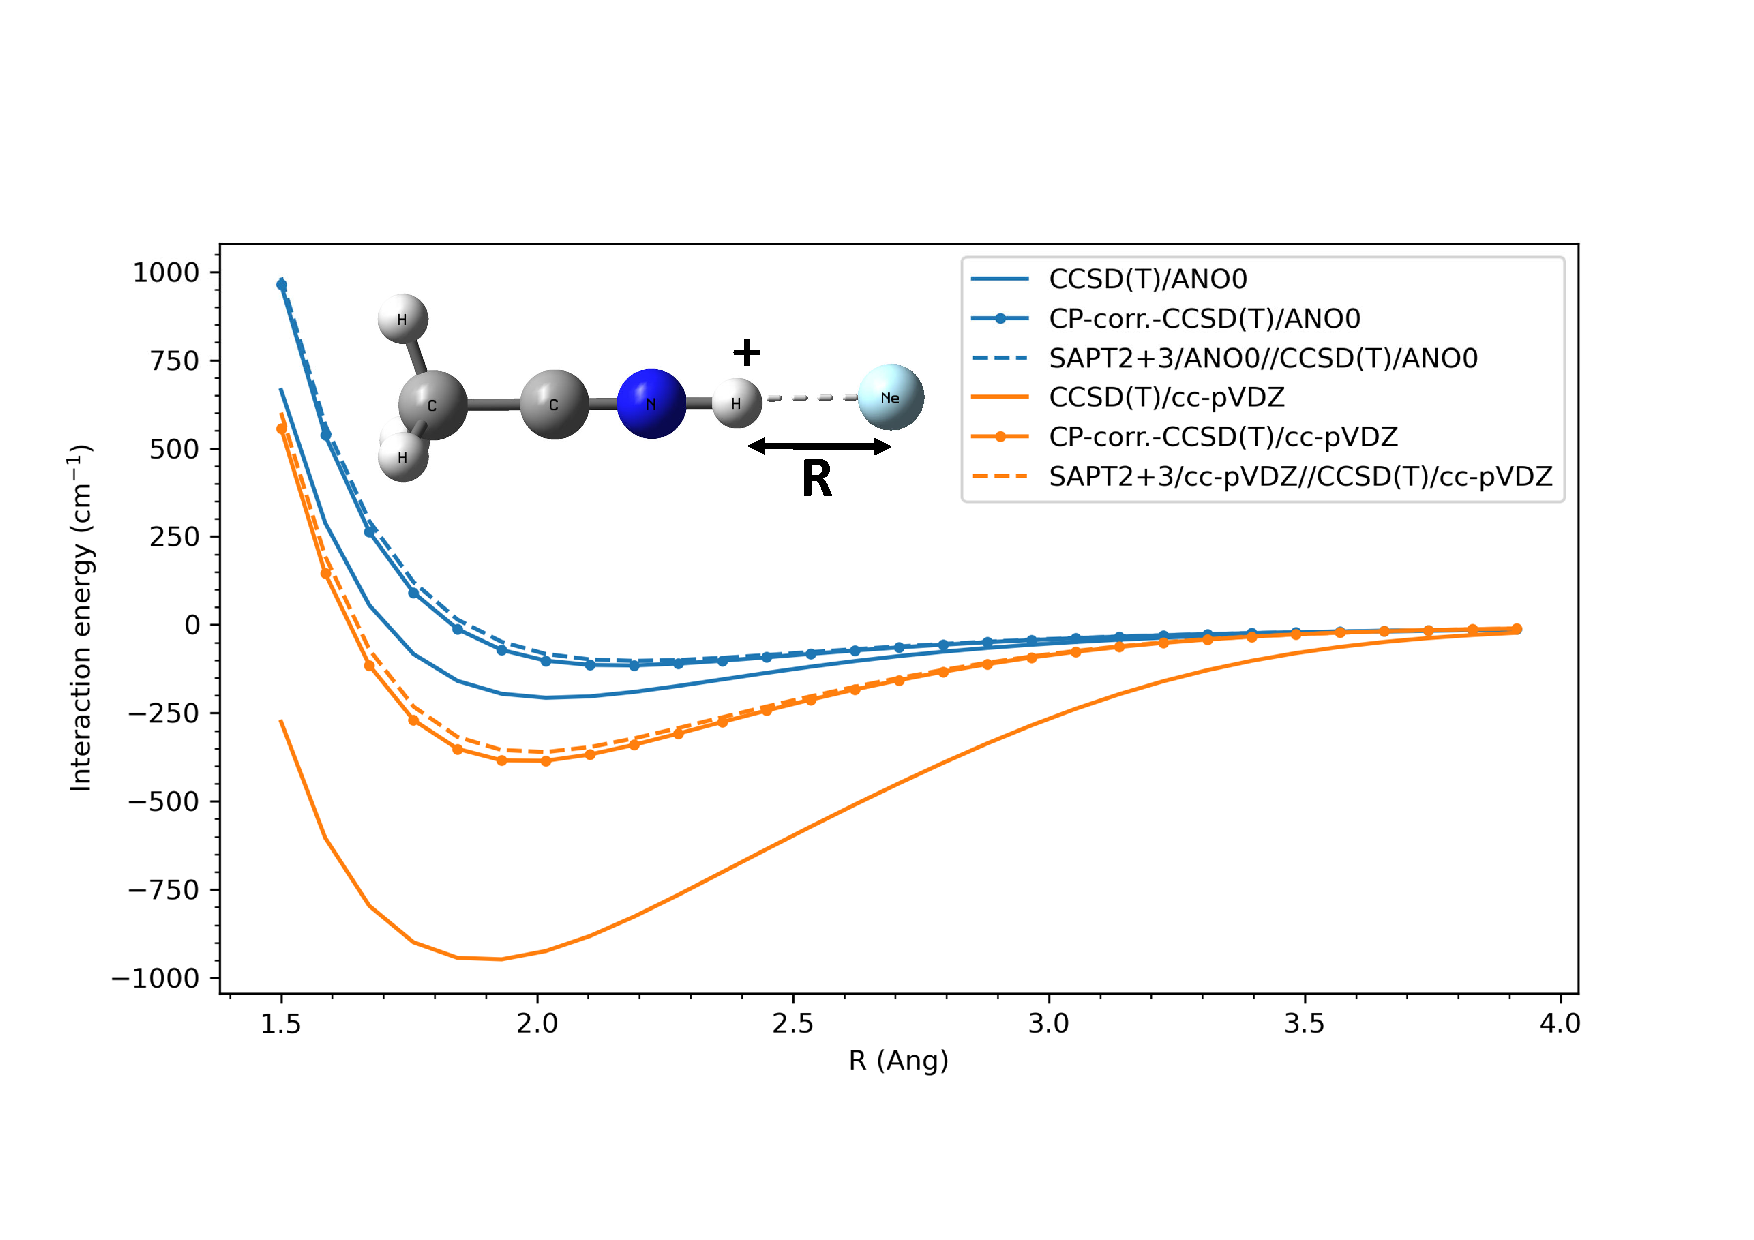
\includegraphics[width=1\textwidth]{chapters/CH3CNH+/figures/iso1_comparison_with_Ne.pdf}
		\caption{Computed potential energy surface as a function of H-Ne distance R for the minimum energy C$_{3v}$ structure of the \pan-Ne complex at various levels of theory.}
	
	\label{FIG:bsse}
\end{figure}
\begin{table}

\caption{Computed binding energies $E_{int}$ or $D_e$, respectively, for the lowest energy \pan-Ne complex ($C_{3v}$ structure) using different BSSE corrections methods. All values are in \wn.}\label{tbl3}
    \centering
    \small
    
    \begin{tabular}{ccccc}

    \\\hline \hline\\
    
        Method          & $D_e$ & CP-corrected: $D_e$ (BSSE) & SAPT2+3: E$_{int}$ \\\\\hline\\
        
        CCSD(T)/ANO0    & -207      & -105 (-102)            & -86               \\
        CCSD(T)/cc-pVDZ & -950      & -378 (-572)            & -348              \\
    
    \\\hline \hline\\
    \end{tabular}
    

\end{table}
\normalsize

Usually, the impact of neon-tagging on vibrational spectra is 
rather small \cite[see, e.g., Ref.][]{Rap2020StableSpectroscopy,Marimuthu2020LaboratorySpectroscopy,Thorwirth2020Molecular+}.
To determine the influence of the neon atom tag on the observed IRPD spectra of \pan, we first searched for the global minimum structure of the \pan-Ne complex. In a first step the geometry of the bare ion was optimized at the CCSD(T)/cc-pVDZ level of theory, and then kept rigid at its equilibrium structure in the following calculations. Potential energy scans were performed at the same level of theory as a function of the distance of the neon ligand from the \pa ion along three trajectories: i) along the molecular symmetry axis, starting from the protonation site, ii) along the CH coordinate of the methyl group, and iii) starting from the nitrogen atom and moving perpendicular to the molecular symmetry axis. The resulting PESs are shown in the Supplementary Information, Figure \ref{fig:CH3CNH+:fig1}, revealing the $C_{3v}$ structure, with the neon atom bound to the proton, to be the global minimum. 

The global minimum structure of the complex was further investigated to account for the Basis Set Superposition Error (BSSE) problem which is a mathematical artefact present in all molecular electronic structure calculations. It is due to the fact that the practical quantum chemical calculations are restricted to the use of finite basis sets \cite{BSSE_Galano2006}. This means that in a complex, the basis sets of the monomers are going to overlap and a situation arises where each atom borrows basis set functions of the other atom, effectively increasing its basis set and therefore stabilizing its energy, i.e. leading to an artificially too deep potential well, as was first observed for the  helium-helium dimer  interaction\cite{BSSE_Kestner1968, liu_accurate_1973}. Since BSSE is strongly geometry dependent, the corresponding PES can substantially differ from the BSSE-free ones  \cite{BSSE_SALVADOR2000}. The usual way to correct for BSSE is based on the counterpoise (CP) scheme introduced by Boys and Bernardi \cite{boys_calculation_1970}. This effect can be clearly noticed in the computed PES as shown in Figure \ref{FIG:bsse}.  The BSSE for comparably sized basis sets, cc-pVDZ and ANO0, are $-572$~\wnn and $-102$~\wn,  respectively (see Table \ref{tbl3}). Additionally, symmetry-adapted perturbation theory (SAPT) which was developed specifically to describe non-covalent interactions between atoms and/or molecules \cite{jeziorski_perturbation_1994, hohenstein_density_2010}, was also computed on the optimized geometry of \pa using the CCSD(T) method with cc-pVDZ and ANO0 basis sets. Since the SAPT computes the interaction energy directly via a pertubative approach, it is inherently BSSE-free as we can also clearly see in Figure \ref{FIG:bsse}. Interestingly the SAPT interaction energy results are very similar to the CP-corrected CCSD(T) (see Figure \ref{FIG:bsse}) while being computationally much more efficient as was also noted in previous studies \cite{SAPT_review2012}. Therefore, to conclude, the ANO0 basis set removes BSSE relatively more efficiently than the corresponding cc-pVDZ (see Figure \ref{FIG:bsse}) and also performs better for frequency calculation (see Table \ref{tab:CH3CNH+:tab3} in the Supplementary Information). This is in agreement with previous studies  \cite{mccaslin_MolPhys_111_1492_2013} where several small poly-atomic molecule's fundamental frequencies were computed at CCSD(T) using both cc-pVXZ(X=D,T,Q) and ANOX(X=0,1,2) basis sets, and compared with experimental results. Here the authors stated that the ANO0 outperforms the similarly sized cc-pVDZ basis sets at least for frequency calculations.

Concluding that CCSD(T) in combination with ANO basis sets provides reliable results for structural calculations of the weakly bound \pan-Ne complex, we calculated its harmonic vibrational frequencies and compared them to those obtained for the bare \pa ion at the CCSD(T)/ANO0 level of theory. The calculated differences in band positions were added to the anharmonic fundamental mode positions of the bare ion obtained at the CCSD(T)/ANO2 level of theory, and are summarized in Table \ref{tbl1:CH3CNH+}. For most modes the complexation with neon leads to band shifts of below 1~\wn, within the uncertainty of the experimental data. An exception are the CNH bending and NH stretching modes, with calculated differences of $+18$ and $-9$~\wn, respectively. This is not surprising, since the binding site of the neon atom is at the N$H$-proton, which is involved in those two vibrational modes, causing a blue and red-shift, respectively, of the bending and stretching bands. Similar but more pronounced effects have been seen for other smaller molecular ions tagged with neon, e.g., HCO$^+$ \cite{NDM1996} and CH$_3^+$ \cite{DOM2000}. It is interesting to note that the corrected frequency for the CNH bending mode now matches the experimental IRPD band position to within its uncertainty. Apart from inducing bandshifts, the IRPD messenger-tagging method can lead to additional bands in the recorded vibrational spectrum caused by combination modes of fundamental modes of the ion core with intramolecular modes involving the neon atom. For the \pan-Ne complex harmonic calculations predict a degenerate bending mode (E) at 32~\wnn and a stretching mode (A$_1$) at 68~\wnn due to vibrations of the neon atom (See Table \ref{tab:CH3CNH+:tab3} in the Supplementary Information). The low-lying bending mode frequency matches well with the frequency difference of weak satellite features observed to the blue of the CCN bending mode (at 414~\wnn), the CNH bending mode (at 611, 620, 644, 664~\wnn), and the CH$_3$ umbrella mode (1388~\wnn). These combination modes might also be responsible for the observed shoulder towards higher frequencies of the CCN bending overtone at 1157~\wn. The long progression of combination bands with multiple excitation of the Ne bending mode seen for the CNH bending mode might be explained by effective dissociation of the \pan-Ne complex upon excitation along the Ne dissociation coordinate, similar effects have been observed previously for other ion ligand complexes \cite{okumura_vibrational_1985,PKB2003,jusko_felion_2019}.

\section{Conclusions}

In this work, we present a comprehensive experimental and quantum-chemical study of the vibrational spectrum of \pan, a potential interstellar molecular ion. Experimental band positions were measured for all fundamental bands, with the exception of the NH stretching band that was studied previously \cite{DRO1999,Amano1992}. The assignment of the corresponding vibrational modes was straightforward based on anharmonic frequency calculations of the bare ion performed at the CCSD(T)/ANO2 level of theory. We could demonstrate that quantum-chemical calculations using the comparatively low-cost ANO0 basis set provide accurate estimates on the influence of the weakly-bound neon atom, used as tag in the IRPD experiments, on the vibrational band positions.\\

The experimental vibrational frequencies obtained in this work provide reliable reference data for infrared astronomical observations to search for protonated methyl cyanide in warmer regions of the ISM or within (exo-)planetary atmospheres, such as that of Titan, where \pa has been mass spectroscopically detected \cite{VYA2006}. The present results also provide a basis for further laboratory studies of \pa at higher resolution in the infrared, e.g., via action spectroscopic schemes like LIICG pioneered in the Schlemmer group \cite{asvany_coltrap_2014,AYB2015}, and for measurements of rotational transitions in its energetically low-lying vibrational states, for which spectroscopic constants are predicted based on high-level quantum-chemical calculations.\\

This work demonstrates once more the versatility of IRPD using weakly bound rare gas atoms as tags, providing vibrational spectra very closely resembling those of the bare ion. However, the proverbial ``innocence" of the neon atom needs to be taken with a grain of salt. For the rather small \pa molecular ion quite substantial shifts $> 10$~\wnn were observed for those vibrational modes that involve the binding site of the neon atom, as also verified by our quantum-chemical calculations. Experiments using helium as tag might be better suited, due to its even lower polarizability and binding energy, as has been demonstrated previously \cite{BKS2003,Dopfer2003,Jasik2013,jusko_felion_2019}. However, for the same reason, i.e. its lower polarizability, He-ion complexes have smaller binding energies, and thus show lower complexation yields, which in turn results in  lower signal-to-noise spectra. Using neon as tagging agent in IRPD is thus a reasonable compromise, and allows in combination with the widely tunable FELIX FELs to uncover broad range vibrational spectra of a large class of molecular ions.
    

% \noindent{\bf Acknowledgements}\\
% We are delighted to contribute this work to the {\it Festschrift for Stephan Schlemmer}. Thanks to Stephan's dedication and enthusiasm the FELion instrument, used for the study of \pa in this work, became a versatile user station at the FELIX Laboratory. We are grateful for his past and continuing support in technical, scientific and personal matters.
% This work is part of the research programme ROSAA with project number 740.018.010, which is (partly) financed by the Netherlands Organisation for Scientific Research (NWO). We gratefully acknowledge the support of Radboud University and of NWO for providing the required beam time at the FELIX laboratory, and the skillful assistance of the FELIX staff. We thank the Cologne Laboratory Astrophysics group for providing the FELion ion trap instrument for the current experiments and the Cologne Center for Terahertz Spectroscopy funded by the Deutsche Forschungsgemeinschaft (DFG, grant SCHL 341/15-1) for supporting its operation. This work was sponsored by NWO
% Exact and Natural Sciences for the use of supercomputer facilities (Grant nr. 2019.062). S.T. acknowledges additional support through the collaborative research center DFG SFB 956 (project ID 184018867, sub-project B2) in Cologne and acknowledges the Regional Computing Center of the Universität zu Köln for providing computing
% time on the DFG funded high-performance computing system CHEOPS. We thank Michael E. Harding for helpful discussions.
% \bibliographystyle{elsarticle-num-names}
% \bibliography{bibtex/allpapers_sorted, bibtex/ref, bibtex/sthorwirth_bibdesk}
% \end{document}

% \section{Internal coordinates of \texorpdfstring{\pa}{CH3CNH+} }


\subsection{fc-CCSD(T)/ANO0}
\begin{verbatim}

H
C 1 r1
C 2 r2 1 a1
X 3 rd 2 a90 1 d0
N 3 r3 4 a90 2 d180
X 5 rd 3 a90 4 d0
H 5 r4 6 a90 3 d180
H 2 r1 3 a1 1 d120
H 2 r1 3 a1 8 d120

r1   =        1.097234034575213
r2   =        1.461586511773973
a1   =      108.354029317585457
rd   =        1.000000409314806
a90  =       89.999999999999972
d0   =        0.000000000000000
r3   =        1.153699023716097
d180 =      180.000000000000000
r4   =        1.013272030286403
d120 =      120.000000000000114

\end{verbatim}
    
\subsection{fc-CCSD(T)/ANO1}

\begin{verbatim}

H
C 1 r1
C 2 r2 1 a1
X 3 rd 2 a90 1 d0
N 3 r3 4 a90 2 d180
X 5 rd 3 a90 4 d0
H 5 r4 6 a90 3 d180
H 2 r1 3 a1 1 d120
H 2 r1 3 a1 8 d120

r1   =        1.091588568955683
r2   =        1.450334012198720
a1   =      108.507798899076860
rd   =        1.000000613972271
a90  =       89.999999999999986
d0   =        0.000000000000000
r3   =        1.145583771122200
d180 =      180.000000000000000
r4   =        1.008294043229717
d120 =      119.999999999999972

\end{verbatim}

\subsection{fc-CCSD(T)/ANO2}
\begin{verbatim}

H
C 1 r1
C 2 r2 1 a1
X 3 rd 2 a90 1 d0
N 3 r3 4 a90 2 d180
X 5 rd 3 a90 4 d0
H 5 r4 6 a90 3 d180
H 2 r1 3 a1 1 d120
H 2 r1 3 a1 8 d120

r1   =        1.090663342780039
r2   =        1.448609574844010
a1   =      108.480759568085148
rd   =        1.000001227944922
a90  =       90.000000000000028
d0   =        0.000000000000000
r3   =        1.142864353443497
d180 =      180.000000000000000
r4   =        1.008334309784723
d120 =      120.000000000000327

\end{verbatim}

\subsection{fc-CCSD(T)/cc-pVDZ}
\begin{verbatim}

H
C 1 r1
C 2 r2 1 a1
X 3 rd 2 a90 1 d0
N 3 r3 4 a90 2 d180
X 5 rd 3 a90 4 d0
H 5 r4 6 a90 3 d180
H 2 r1 3 a1 1 d120
H 2 r1 3 a1 8 d120

r1   =        1.104421287381395
r2   =        1.467855029147642
a1   =      108.258731223153745
rd   =        1.000000409314806
a90  =       89.999999999999957
d0   =        0.000000000000000
r3   =        1.160263599078930
d180 =      180.000000000000000
r4   =        1.020376191984162
d120 =      120.000000000000171

\end{verbatim}

\subsection{fc-CCSD(T)/cc-pVTZ}
\begin{verbatim}

H
C 1 r1
C 2 r2 1 a1
X 3 rd 2 a90 1 d0
N 3 r3 4 a90 2 d180
X 5 rd 3 a90 4 d0
H 5 r4 6 a90 3 d180
H 2 r1 3 a1 1 d120
H 2 r1 3 a1 8 d120

r1   =        1.091362895166567
r2   =        1.453075807535473
a1   =      108.438787022956490
rd   =        1.000000204657382
a90  =       89.999999999999986
d0   =        0.000000000000000
r3   =        1.146078556823367
d180 =      180.000000000000000
r4   =        1.009021121407080
d120 =      120.000000000000099

\end{verbatim}

\subsection{ae-CCSD(T)/cc-pwCV5Z}
\begin{verbatim}

H
N 1 r1*
X 2 rd 1 a90
C 2 r2* 3 a90 1 d180
X 4 rd 2 a90 3 d0
C 4 r3* 5 a90 2 d180
H 6 r4* 4 a1* 5 d0
H 6 r4* 4 a1* 7 d120
H 6 r4* 4 a1* 8 d120

r1   =        1.0073314907
rd   =        1.0
a90  =       90.0
r2   =        1.1399556988
d180 =      180.000000000000000
d0   =        0.000000000000000
r3   =        1.4440897526
r4   =        1.0887809197
a1   =      108.5586585536
d120 =      120.0

\end{verbatim}

\section{Internal coordinates of \texorpdfstring{\pan}{CH3CNH+} -Ne }

\subsection{fc-CCSD(T)/ANO0}

\begin{verbatim}

H
C 1 r1
C 2 r2 1 a1
X 3 rd 2 a90 1 d0
N 3 r3 4 a90 2 d180
X 5 rd 3 a90 4 d0
H 5 r4 6 a90 3 d180
H 2 r1 3 a1 1 d120
H 2 r1 3 a1 8 d120
X 7 rd 5 a90 6 d0
NE 7 r5 10 a90 5 d180

r1   =        1.097234259132258
r2   =        1.461586810898442
a1   =      108.354029317585457
rd   =        1.000000613972271
a90  =       89.999999999999972
d0   =        0.000000000000000
r3   =        1.153699259829119
d180 =      180.000000000000000
r4   =        1.013272237660004
d120 =      119.999999999999758
r5   =        2.117272059249112

\end{verbatim}

\subsection{fc-CCSD(T)/cc-pVDZ}
\begin{verbatim}

H
C 1 r1
C 2 r2 1 a1
X 3 rd 2 a90 1 d0
N 3 r3 4 a90 2 d180
X 5 rd 3 a90 4 d0
H 5 r4 6 a90 3 d180
H 2 r1 3 a1 1 d120
H 2 r1 3 a1 8 d120
X 7 rd 5 a90 6 d0
NE 7 r5 10 a90 5 d180

r1   =        1.097234483689349
r2   =        1.461587110022973
a1   =      108.354029317585457
rd   =        1.000000818629779
a90  =       89.999999999999972
d0   =        0.000000000000000
r3   =        1.153699495942189
d180 =      180.000000000000000
r4   =        1.013272445033648
d120 =      119.999999999999758
r5   =        1.990534530346215
\end{verbatim}
\newpage

\newgeometry{left=2.5cm}
% \section{Computed vibrational frequencies}

\begin{landscape}
\begin{center}
\begin{table}[h]
\caption{Computed fc-CCSD(T) vibrational frequencies (in \wn) using ANO basis sets for \pa. }\label{tab:CH3CNH+:tab1}

    \begin{tabular}{llllllllll} \hline\hline\\
            mode        & sym      & exp.$^a$ & \multicolumn{3}{c}{harmonic$^b$}  & \multicolumn{3}{c}{anharmonic (VPT2)$^b$} \\
                        & C$_{3v}$ &      & ANO0        & ANO1       & ANO2       & ANO0        & ANO1      & ANO2 &          \\\hline\\
            $\nu_{10}$  & E	       & 385  & 374 (-11)	& 381  (-4)  & 382  (-3)  & 376  (-9)   & 384 (-1)  & 384  (-1)       \\
            $\nu_9$     & E	       & 596  & 581 (-15)	& 580  (-16) & 585  (-11) & 570  (-26)  & 579 (-17) & 577  (-19)      \\
            $\nu_5$     & A$_1$	   & 898  & 889 (-9)	& 897  (-1)  & 900  (2)   & 878  (-20)  & 887 (-11) & 890  (-8)       \\
            $\nu_8$     & E	       & 1026 & 1051 (25)	& 1048 (22)  & 1050 (24)  & 1025 (-1)   & 1023(-3)  & 1024 (-2)       \\
            $\nu_4$     & A$_1$	   & 1364 & 1395 (31)	& 1393 (29)  & 1398 (34)  & 1358 (-6)   & 1358(-6)  & 1361 (-3)       \\
            $\nu_7$     & E	       & 1421 & 1444 (23)	& 1442 (21)  & 1447 (26)  & 1422 (1)    & 1428(7)   & 1429 (8)        \\
            $\nu_3$     & A$_1$	   & 2307 & 2336 (29)	& 2345 (38)  & 2350 (43)  & 2290 (-17)  & 2300(-7)  & 2305 (-2)       \\
            $\nu_2$     & A$_1$	   & 2924 & 3060 (136)	& 3049 (125) & 3051 (127) & 2934 (10)   & 2927(3)   & 2930 (6)        \\
            $\nu_6$     & E	       & 2996 & 3174 (178)	& 3149 (153) & 3152 (156) & 3019 (23)   & 2999(3)   & 3002 (6)        \\
            $\nu_1$     & A$_1$	   & nc   & 3688 (-)	& 3699 (-)	 & 3687 (-)   & 3528 (-)    & 3534(-)   & 3525 (-)        \\
        \\
        \hline\hline\\
    \end{tabular}
    
    $^a$ This work, Ne-IRPD experiment.\\
    $^b$ Shift from Ne-IRPD experiment is given in parenthesis.
\end{table}
\end{center}
\end{landscape}
\restoregeometry

\begin{table}[h]
\caption{Computed harmonic CCSD(T) vibrational frequencies (in \wn) using Dunning's basis sets for \pa. }\label{tab:CH3CNH+:tab2}
\begin{center}
    \begin{tabular}{llllll} \hline\hline\\
       mode         & sym.  & exp.$^a$  & cc-pVDZ$^b$ & cc-pVTZ$^b$ \\\hline\\
       $\nu_{10}$   & E	    & 385       & 362  (-23)	  & 380  (-5)    \\
       $\nu_9$      & E	    & 596       & 564  (-32)	  & 586  (-10)   \\
       $\nu_5$      & A$_1$	& 898       & 893  (-5)	  & 895  (-3)    \\
       $\nu_8$\     & E	    & 1026      & 1042 (15)  & 1052 (25)  \\
       $\nu_4$      & A$_1$	& 1364      & 1381 (16)  & 1398 (34)  \\
       $\nu_7$      & E	    & 1421      & 1433 (12)  & 1450 (29)  \\
       $\nu_3$      & A$_1$	& 2307      & 2331 (24)  & 2343 (36)  \\
       $\nu_2$      & A$_1$	& 2924      & 3066 (142) & 3052 (128) \\
       $\nu_6$      & E	    & 2996      & 3181 (185) & 3151 (154) \\
       $\nu_1$      & A$_1$	& nc        & 3663 (-)	  & 3684 (-)    \\
        \\
        \hline\hline\\
    \end{tabular}
    
    $^a$ This work, Ne-IRPD experiment.\\
    $^b$ Shift from Ne-IRPD experiment is given in parenthesis.
\end{center}

\end{table}

\begin{table}
\footnotesize
\caption{Computed harmonic CCSD(T) vibrational frequencies (in \wn) comparing both \pa (bare ion) and \pan-Ne (complex) using ANO0 and cc-pVDZ basis sets. }\label{tab:CH3CNH+:tab3}

\begin{center}
    \begin{tabular}{lllllll} \hline\hline\\
    
        mode                    & sym.      & exp.$^a$ & \multicolumn{2}{c}{ANO0$^b$} & \multicolumn{2}{c}{cc-pVDZ$^b$}\\
                                & C$_{3v}$  &      & \pa          & \pan-Ne     & \pa         & \pan-Ne \\ \hline\\
        $\nu_{\mbox{Ne-bend}}$  & E	        &      &              & 32 & 	                 & 26           \\
        $\nu_{\mbox{Ne-str.}}$  & A$_1$	    &      &              & 68 & 	                 & 102          \\
        $\nu_{10}$              & E	        & 385  &  374  (-11)  & 375  (-10) & 362  (-23)	 & 322  (-63)   \\
        $\nu_9$                 & E	        & 596  &  581  (-15)  & 599  (3)   & 564  (-32)	 & 551  (-45)   \\
        $\nu_5$                 & A$_1$	    & 898  &  889  (-9)   & 890  (-8)  & 893  (-5)	 & 913  (15)    \\
        $\nu_8$                 & E	        & 1026 &  1051 (25)   & 1052 (26)  & 1042 (15)	 & 1024 (-2)    \\
        $\nu_4$                 & A$_1$	    & 1364 &  1395 (31)   & 1395 (31)  & 1381 (16)	 & 1370 (6)     \\
        $\nu_7$                 & E	        & 1421 &  1444 (23)   & 1445 (24)  & 1433 (12)	 & 1425 (4)     \\
        $\nu_3$                 & A$_1$	    & 2307 &  2336 (29)   & 2336 (29)  & 2331 (24)	 & 2380 (73)    \\
        $\nu_2$                 & A$_1$	    & 2924 &  3060 (136)  & 3060 (136) & 3066 (142) & 3129 (205)   \\
        $\nu_6$                 & E	        & 2996 &  3174 (178)  & 3173 (177) & 3181 (185) & 3247 (251)   \\
        $\nu_1$                 & A$_1$	    & nc   &  3688 (-)    & 3679 (-)   & 3663 (-)	 & 3730 (-)	    \\

        \\\hline\hline\\
    \end{tabular}\\
    $^a$ This work, Ne-IRPD experiment.\\
    $^b$ Shift from Ne-IRPD experiment is given in parenthesis.
    
\end{center}
\end{table}

\begin{figure}
	\centering
		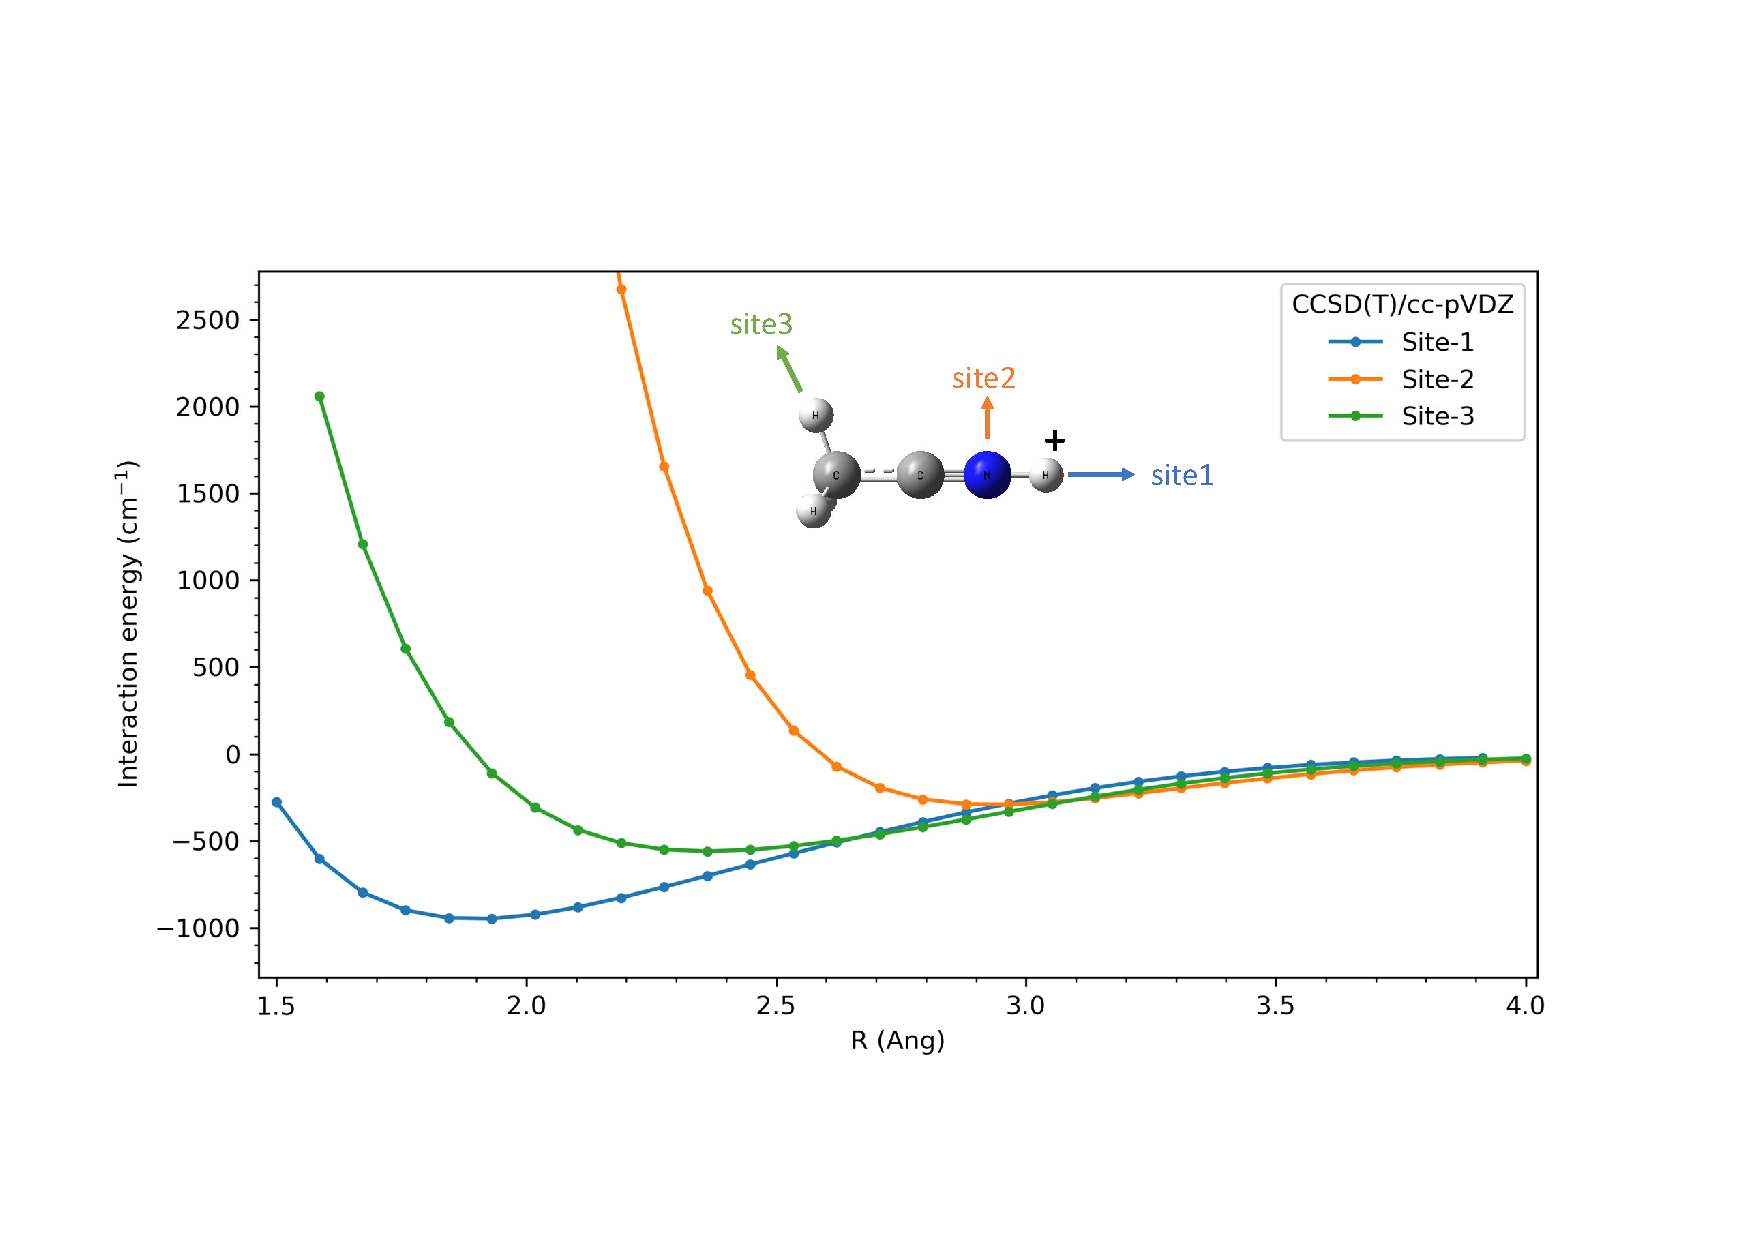
\includegraphics[width=1\textwidth]{chapters/CH3CNH+/figures/iso_comparison_with_Ne.pdf}
		\caption{Computed potential energy surface as a function of Ne distance R for \pan-Ne from various sites neon atom placed.}\label{fig:CH3CNH+:fig1}
	% \label{FIG:bsse}
\end{figure}

\begin{figure}

	\centering
		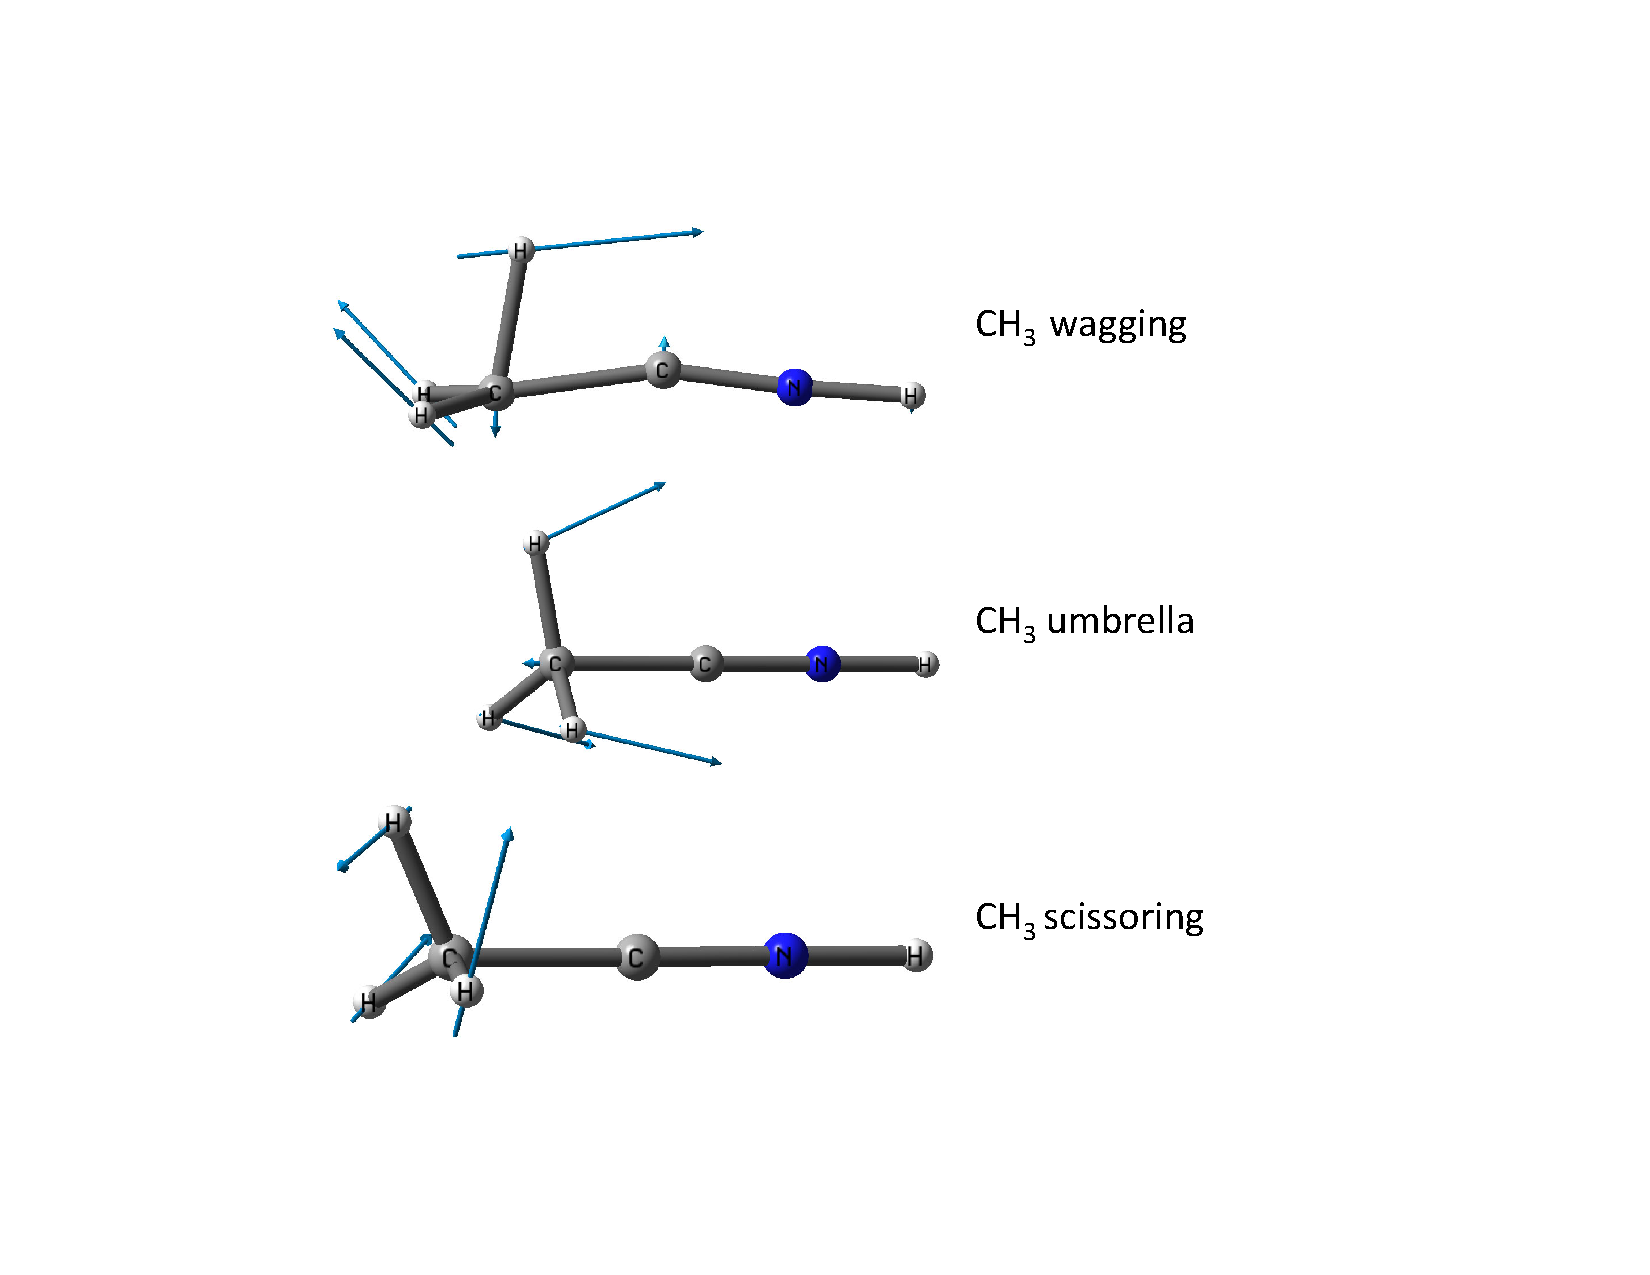
\includegraphics[scale=.5]{chapters/CH3CNH+/figures/vibration_vector.pdf}
		\caption{Vibrational displacement vectors for CH$_3$ modes.}\label{fig:CH3CNH+:fig2}
	\label{FIG:ch3_modes}
\end{figure}

\newpage
% \section{Calculated rotational spectroscopic parameters\\ at the CCSD(T)/ANO2 level of theory}

\begin{center}
    \begin{table}[h]
    \caption{Calculated spectroscopic parameters of \pa at the CCSD(T)/ANO2 level of theory. Rotational constants $B_e$, $B_0$, $\Delta B_0=1/2\Sigma \alpha^B_i$ ($\Delta A_0$ analogous), and $\alpha^A_i$ and $\alpha^B_i$. All values are in MHz.}\label{tab:CH3CNH+:tab4}
        \centering
        \begin{tabular}{cccccc}
            \hline\hline\\
            $A_e$    & $A_0$    &  $\Delta A_0$ & $B_e$  & $B_0$  & $\Delta B_0$  \\\hline\\
            156213.5 & 154336.7 & 1876.8        & 8659.2 & 8541.5 & 27.8            \\\\
            \hline\hline\\
            \multicolumn{2}{c}{mode}          & $\alpha^A_i$ & $\alpha ^B_i$ & $q_i$ & \\\hline\\
            $\nu_{10}$ & CCN bend             & 91.3  &  -20.2 & 14.8    &  \\
            $\nu_9$    & CNH bend             & 31.1  &  -8.3  & 8.9     &  \\
            $\nu_5$    & CC stretch           & 251   &  50.6  &         &  \\
            $\nu_8$    & CH$_3$ wagging       & -883  &  -0.09 & 3.6     &  \\
            $\nu_4$    & CH$_3$ umbrella      & -912  &  68.0  &         &  \\
            $\nu_7$    & CH$_3$ scissoring    & 902   &  -37.7 & 60.2    &  \\
            $\nu_3$    & CN stretch & 103     & 44.0  &        &            \\
            $\nu_2$    & CH$_3$ sym. stretch  & 1645  & 2.2    &         &  \\
            $\nu_6$    & CH$_3$ asym. stretch & 1204  & 0.99   & 0.634   &  \\
            $\nu_1$    & NH stretch           & -23.4 & 21.5   &         &  \\
            
            \hline\hline
        \end{tabular}
        \label{rot}
    \end{table}
\end{center}
% \end{subappendices}

